\subsection{Закон Амдала, его следствия. Граф алгоритма. Критический путь графа алгоритма, ярусно-параллельная форма графа алгоритма. Этапы решения задач на параллельных вычислительных системах.}


\textbf{Ускорение}, получаемое при использовании параллельного алгоритма для $p$ процессоров выражается: $S = \frac{T_1}{T_p}$, где $T_1$ --- время выполнения задачи на одном процессоре, $T_p$ --- время параллельного выполнения задачи на $p$ процессорах.

\textbf{Закон Амдала}:
$S \leqslant \frac{1}{f + \frac{1 - f}{p}}$, где

$f$ --- доля операций, которые обязаны быть выполнены последовательно ($0 \leqslant f \leqslant 1$), 

$p$ --- число процессоров.

\textbf{Следствие 1.} 
Для того чтобы ускорить программу в $q$ раз, необходимо не менее, чем в $q$ раз, ускорить не менее, чем $\left(1 - \frac{1}{q}\right)$-ю часть программы. Это необходимое, но не достаточное условие.

\textbf{Следствие 2.} (при большом числе процессоров): 
$S \approx \frac{1}{f}$.

\textbf{Граф алгоритма}

Будем представлять программы с помощью графов.

\textbf{Граф алгоритма}-- ориентированный граф, состоящий из вершин, соответствующих операциям алгоритма, и направленных дуг, соответствующих передаче данных (результаты одних операций передаются в качестве аргументов другим операциям) между ними. Не следует путать его с графом управления программы и тем более с её блок-схемой.

Вершины: процедуры, циклы, линейные участки, операторы, итерации циклов, срабатывания операторов. 

Операции -- одна вершина для каждой операции. 

Срабатывания операторов -- столько вершин, сколько раз каждый оператор сработал.

Дуги: отражают связь (отношение) между вершинами.

Особенностями графа алгоритма являются:

 - его ацикличность, нет кратных дуг;
 
 - невозможность, в общем случае, его описания простым перечислением, в силу того, что его составляющие могут зависеть от внешних параметров решаемой им задачи (например, алгоритм, реализующий метод Гаусса — от размера матрицы)

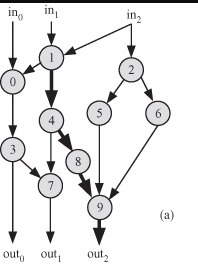
\includegraphics[width=0.6\columnwidth]{pics/dop09_graph.png}

Выделяют два типа отношений: операционное и информационное.

\textbf{Операционное отношение}: две вершины A и B соединяются направленной дугой $A \Rightarrow B$ тогда и только тогда, когда вершина $B$ может быть выполнена сразу после вершины $A$.

\textbf{Информационное отношение}: две вершины $A$ и $B$ соединяются направленной дугой $A \Rightarrow B$ тогда и только тогда, когда вершина $B$ использует в качестве аргумента некоторое значение, полученное в вершине $A$.

\bigbreak
\textbf{Операционный граф}: вершины --- операции, дуги --- операционные отношения.

\textbf{Граф операционной истории программы}: вершины --- срабатывания операторов, дуги --- операционные отношения.

\textbf{Информационный граф}: вершины --- операции, дуги --- информационные отношения.

\textbf{Граф информационной истории программы}: вершины --- срабатывания операторов, дуги --- информационные отношения. 

Независимо от способа построения ориентированного графа, те его вершины, которые не имеют ни одной входящей или выходящей дуги, будем называть соответственно \textbf{входными} или \textbf{выходными вершинами} графа.


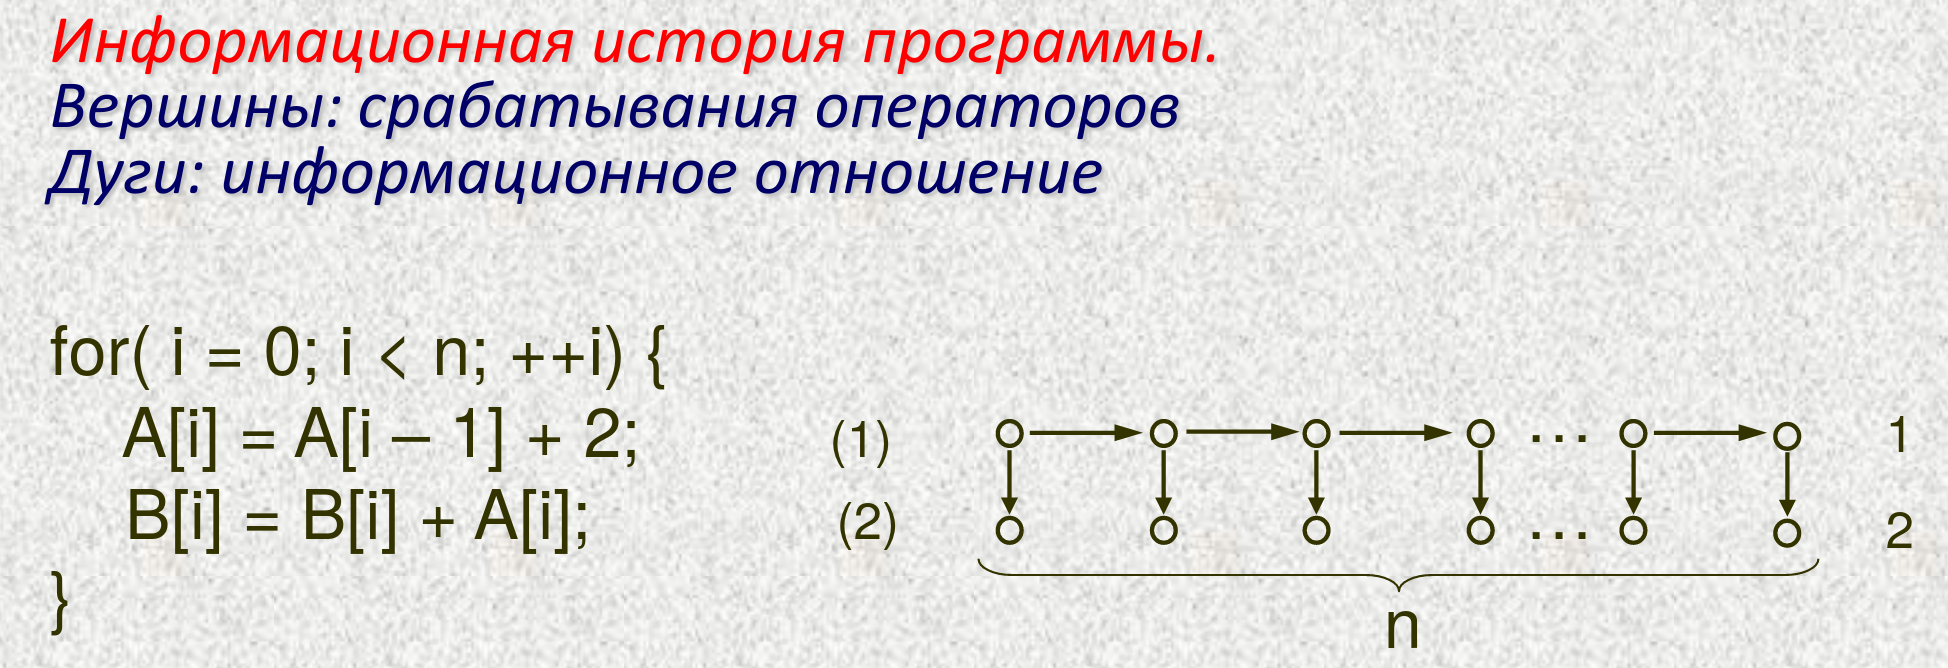
\includegraphics[width=\columnwidth]{pics/inf_hystory.png}

\textbf{Критический путь графа алгоритма} --- это длина самого длинного пути от <входа> графа к его <выходу> (от первого оператора к последнему).

\textbf{Ярусно-параллельная форма графа алгоритма} позволяет описать ресурс параллелизма программ и алгоритмов.
\begin{itemize}
    \item Начальная вершина каждой дуги расположена на ярусе с номером меньшим, чем номер яруса конечной вершины.
    \item Между вершинами, расположенными на одном ярусе, не может быть дуг.
\end{itemize}

\textbf{Высота ЯПФ} --- это число ярусов 

\textbf{Ширина яруса} --- число вершин, расположенных на ярусе

\textbf{Ширина ЯПФ} --- это максимальная ширина ярусов в ЯПФ.

Высота ярусно-параллельной формы --- это сложность параллельной реализации алгоритма/программы. 
ЯПФ определяется неоднозначно. 

Ярусно-параллельная форма называется \textbf{канонической}, если у любой вершины, кроме вершин первого яруса, есть входная дуга, идущая с предыдущего яруса. 
Высота канонической ЯПФ = длине критического пути + 1.

\textbf{Этапы решения задач на параллельных вычислительных системах}
\todo{Это точно то о чем спрашивается?}
Решение задачи на параллельной вычислительной системе будет эффективным только в том случае, если на всем пути от Задачи до Компьютера не возникнет ни одного <узкого места>.
Центральная проблема: отображение программ и алгоритмов на архитектуру параллельных вычислительных систем (Co-Design).

Весь процесс решения некоторой задачи на параллельной  ВС можно разбить на следующие этапы: 
\begin{enumerate}
    \item Формулировка задачи.
    \item Составление модели исследуемого в задаче объекта.
    \item Определение метода решения задачи для получения необходимой результирующей информации на основании используемой модели.
    \item Разработка алгоритма решения задачи на основе используемого метода и модели исследуемого в задаче объекта.
    \item Выбор технологии программирования.
    \item Разработка программы для соответствующей параллельной ВС на основе имеющегося алгоритма и получение результирующей информации после выполнения программы.
\end{enumerate}


% -------- source --------
\bigbreak
[\cite[page 69-96]{replace_me}]